\chapter{Methodology}~\label{chap:met}

Literature Review chapter~(\ref{chap:lr}) defines current approaches to solve the task of Commit Messages Generation\textbf{(CMG)}. It includes deep learning models, used for generating messages, datasets constructed for this purpose, and metrics typically used to evaluate the model performance. In this chapter, I'm aiming to describe the steps I took to achieve the goal from the Introduction chapter~(\ref{chap:intro}). Section~\ref{sec:experiment_design} describes the overall structure of conducted experiments and precisely defines the goal of the work. In Section~\ref{sec:data_retrieval} I will precisely describe the process of constructing a dataset of commits, including data collecting and scrubbing of data outliers.

\section{Experiment design}~\label{sec:experiment_design}
The main objective of this study is to develop a system for automatically generating commit messages that rival state-of-the-art (SOTA) methods. To achieve this, I first need to construct my dataset. The next step involves analyzing this data and that from other studies, crucial for understanding the data structure and extracting relevant statistics. This analysis also involves filtering to ensure data quality. Subsequently, my research will examine the metrics used in Neural Machine Translation (NMT) tasks, requiring an understanding of their calculation methods and underlying intuition. Finally, I will train various models, providing a detailed description of each model's architecture and the rationale for its expected success in the commit message generation (CMG) task.

\section{Data retrieval}~\label{sec:data_retrieval}
The first step I took in my work was to get the data from open sources. In the task of the automatic commit messages generation, the data to train or evaluate the models should be in the format of labelled pairs code changes and the corresponding commit message.
\subsection{Retrieval process}
 To get the data I decided to parse the most starred GitHub\footnote[1]{\href{https://github.com}{GitHub: Cloud storage for code projects.}} repositories which were mostly written in Python programming language. For this purpose, I first get the names of the repositories and links for them via GitHub API\@. One way of getting the commits content from the repository is directly using the GitHub API, but due to the API calls limit I decided to do this in another way. With the use of the GitPython\footnote[2]{\href{https://pypi.org/project/GitPython/}{Description of the library}}, which is a python library used to interact with git repositories I firstly cloned all the repositories from the retrieved list into my local machine and then fetch the information about all the commits from the \texttt{.git} directory. 

 \subsection{Retrieved components}
 The main components of the data sample are the code changes and corresponding commit messages. However, for further research, I included some additional fields in my dataset. At the end of the data parsing process, I came up with the features, mentioned in the table~{}\ref{table:commit_data_attributes}

{ 
    \renewcommand{\arraystretch}{2} % Change 1.5 to whatever multiplier you want
    \begin{table}[h]
    \caption{Commit Data Attributes}\label{table:commit_data_attributes}
    \centering
    \begin{tabularx}{\textwidth}{|l|X|} % % chktex 44
    \hline % chktex 44
    \textbf{Attribute} & \textbf{Description} \\
    \hline % chktex 44
    Name of repository & Name of the project in which the current commit was added. Useful for associating the commit with its project. \\
    \hline % chktex 44
    Commit message & Label for the prediction that will be used by the model in the training phase. \\
    \hline % chktex 44
    Commit changes & Input data for the model. \\
    \hline % chktex 44
    Number of changed files in the commit & Statistics about the retrieved data. \\
    \hline % chktex 44
    Length of code changes in chars & Statistics about the retrieved data. \\
    \hline % chktex 44
    Hash of the commit & Unique identifier for the current commit to avoid duplicates. \\
    \hline % chktex 44
    \end{tabularx}
\end{table}
}
    
    

 \subsection{Structure of the data}~\label{sec:structure_of_the_data}
 Before passing data to the Deep Learning model we first need to preprocess it. For my task, I decided to add some special tokens to the code changes and commit messages. 
 I used the following special tokens:
\begin{itemize}
    \item \verb+<file_name>+ for the name of the file before and after the commit
    \item \verb+<code_del>+ for code lines deleted in the commit
    \item \verb+<code_add>+ for code lines added in the commit
    \item \verb+<commit_msg>+ for the commit message
\end{itemize}
These special tokens are used to separate the most important parts of the input. Tokens described above are used at the beginning of the line, and the opposite with a backslash is used to signify the end of this part. The final format of the model input data is the following:
 
 \begin{verbatim}
    <file_name> old file name </file_name>
    <file_name> new file name </file_name>
    <code_del> deleted code </code_del>
    <code_add> added code </code_add>
    <commit_msg> commit message </commit_msg>
\end{verbatim}
\section{Collected data analysis and filtering}~\label{sec:data_analysis}
For my dataset, I collected the data from 400 most-starred GitHub repositories. But due to the repetitions at the end, I came up with \textasciitilde{}300 thousand commit samples from 311 different repositories with in total \textasciitilde{}1.2 million code files changed. Fig~\ref{fig:commits_distribution} shows the distribution of the number of commits among the repositories I took from GitHub. It does not include some data outliers, where the number of commits is too big. From this histogram, we can conclude that in average repository has \textasciitilde{}3000 commits. 
\begin{figure}[H]
    % \hspace*{-2.5cm}
    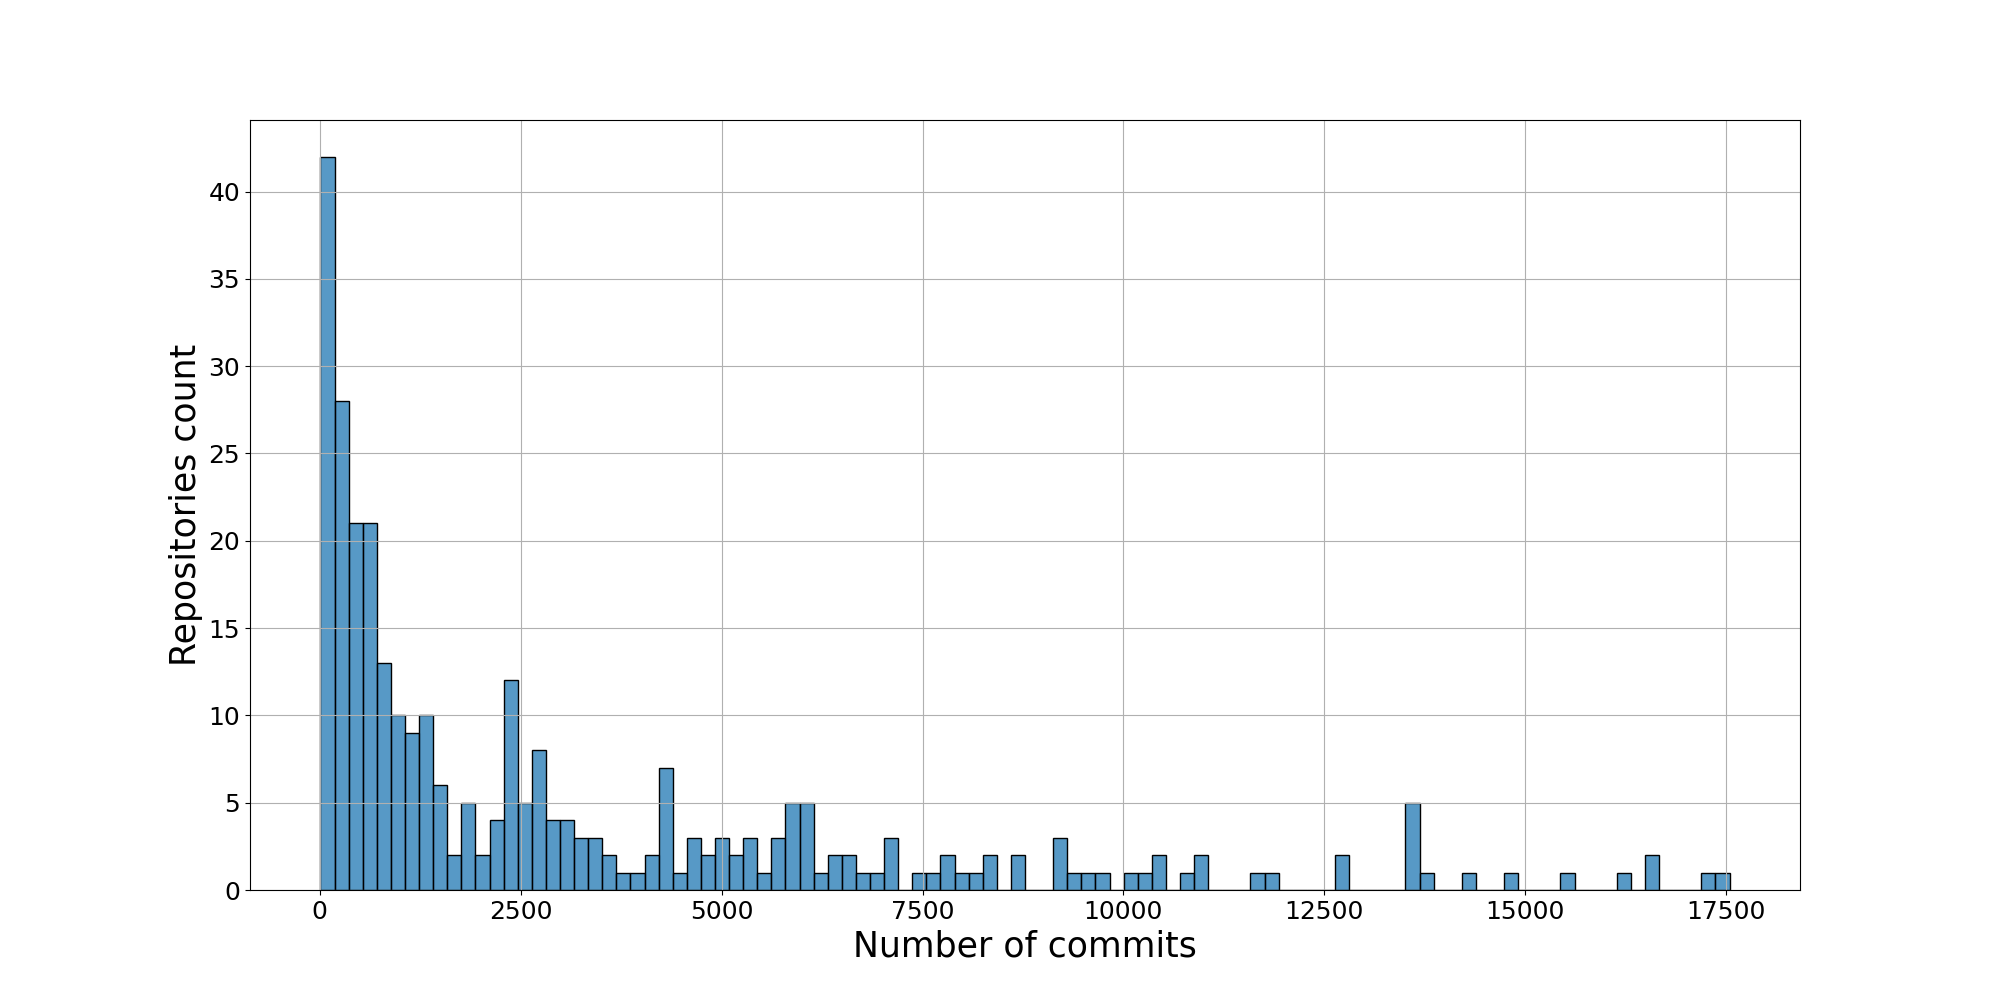
\includegraphics[scale=0.30]{figs/Commits distribution.png}
    \caption{Distribution of the number of commits in the repositories.}~\label{fig:commits_distribution}
\end{figure}

\begin{figure}[H]
    % \hspace*{-2.5cm}
    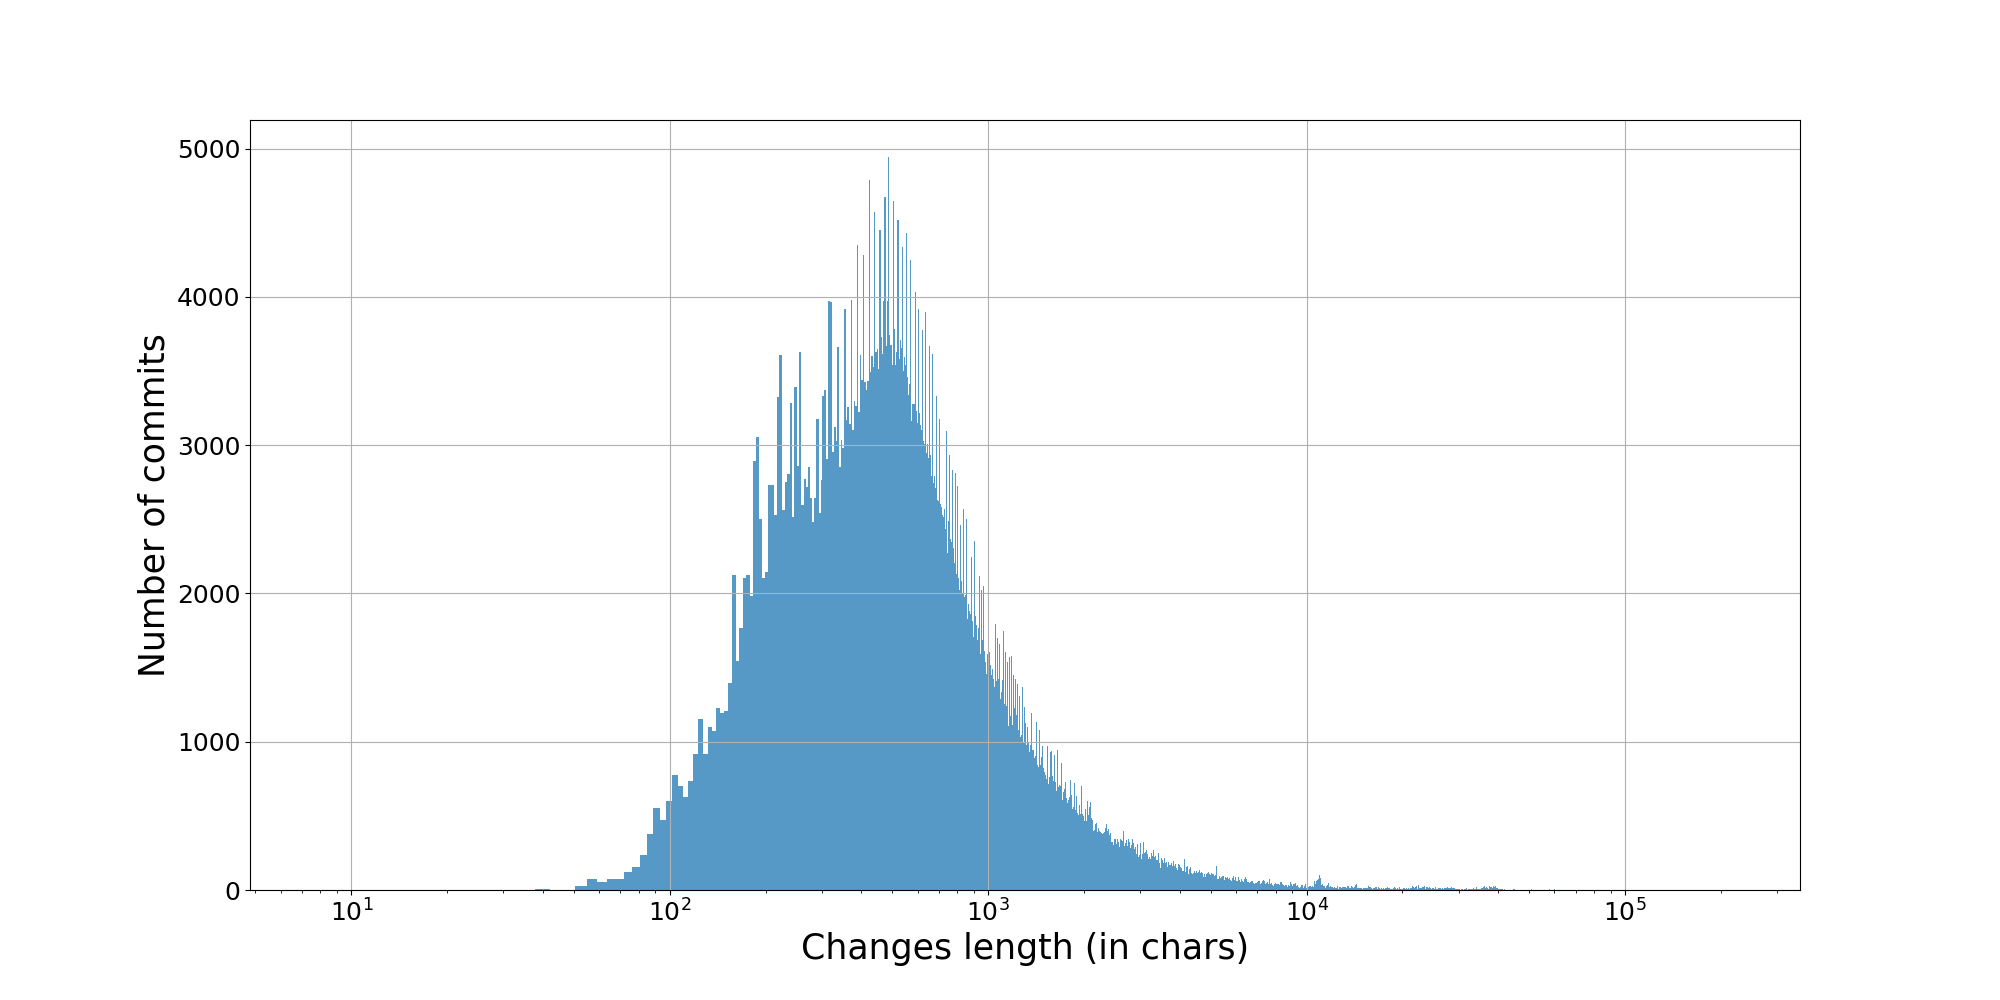
\includegraphics[scale=0.30]{figs/changes_len_dist.png}
    \caption{Distribution length of the commits in the dataset.}~\label{fig:changes_len_dist}
\end{figure}
Fig~\ref{fig:changes_len_dist} represents the distribution of the code changes in commits. From this distribution, we can see that the average length of the code changes is \textasciitilde{}5000 characters. From this, we can conclude that the code changes on average in a very long sequence. Most of the modern Deep Learning models are transformer-based and therefore experience significant degradation of the performance due to the quadratic complexity of the self-attention mechanism as mentioned in {}\cite{keles2023computational}. Also in this step, I decided to trim my dataset, to have only samples with less than 6000 characters. With this truncation, we lose only 15\% of the data but have much shorter sequences on average.
% chktex -o 44
\begin{figure}[H]
    % \hspace*{-2.5cm}
    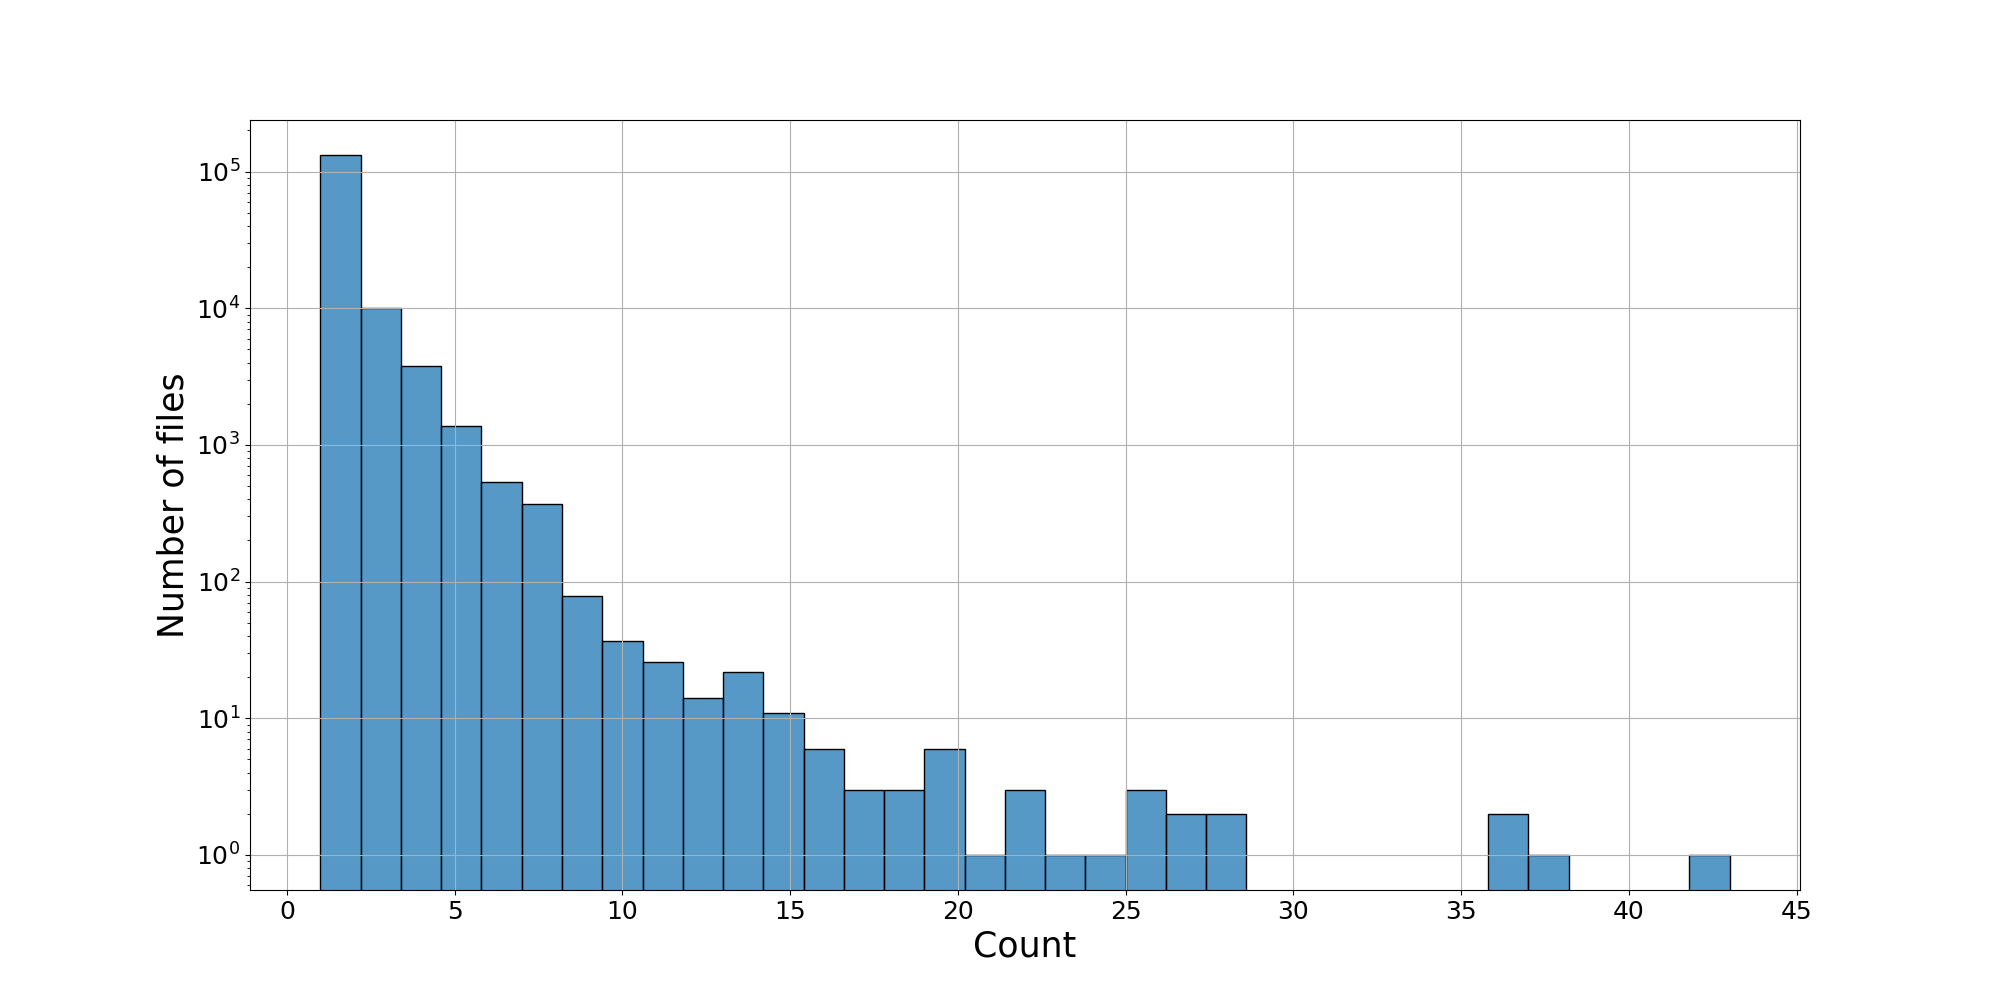
\includegraphics[scale=0.30]{figs/Commit num files distribution.png}
    \caption{Distribution of the number of files in commits.}~\label{fig:Commit num files distribution}
\end{figure}

Figure~{}\ref{fig:Commit num files distribution} shows how commits in my dataset are distributed based on the number of files they modify. From this histogram, we can see what significant number of commits change more than one file. To be precise, single file commits are two-thirds of all data samples. 

One more insight, that we can get from the collected data is the most popular beginning word of commit messages. This part of the data analysis is similar to the one from~{}\cite{jung2021commitbert}. The authors of this work state that commit typically states with the common verbs. From the collected dataset I extracted the 10 most used starting words for commits and got the results, presented in the table~{}\ref{tab:commit_messages}. From this table, it's visible that there exist some common words for starting a commit message. Even among these 10 words, there are several repetitive ones with modified writing or form. These words cover \textasciitilde{}35\% of the total number of samples in the dataset.
\begin{table}[h]
    \centering
    \begin{tabular}{|l|r|} % chktex 44
    \hline % chktex 44
    \textbf{Commit Message} & \textbf{Count} \\ 
    \hline % chktex 44
    Merge     & 25313 \\ \hline % chktex 44
    Fix       & 17891 \\ \hline % chktex 44
    Add       & 15476 \\ \hline % chktex 44
    Update    & 10473 \\ \hline % chktex 44
    Issue     & 7979  \\ \hline % chktex 44
    Added     & 7514  \\ \hline % chktex 44
    fix       & 6496  \\ \hline % chktex 44
    add       & 5600  \\ \hline % chktex 44
    Remove    & 5328  \\ \hline % chktex 44
    Fixed     & 4820  \\ \hline % chktex 44
    \end{tabular}
    \caption{Distribution of commit messages}\label{tab:commit_messages}
\end{table}

In the data filtering step my goal was to get rid of too long samples and samples with bad quality commit messages, which may lead to the model degradation. After all, I came up with the following filtering criteria: 
\begin{itemize}
    \item Samples with too long code changes (more than 6000 characters, 85 percentile).
    \item Samples from repositories with too many commits
    \item Samples with too long commit messages (more than 950 characters, 98 percentile).
    \item Samples with non-ASCII symbols in the commit message.
    \item Samples without Python code changes.
\end{itemize}
The filtered dataset I got, in the end, is made of \textasciitilde{}300 thousand commits from 170 repositories. 

\section{Analysis of datasets from other works}
In the literature review chapter~(\ref{chap:lr}) I described most of the existing datasets for the commit messages generation task. But in this section, I would like to focus only on the CommitChronicle dataset, presented in {}\cite{eliseeva2023commit}. It consists of 10.7M commits in 20 programming languages from 11.9k GitHub repositories. It also includes not only code changes with the corresponding commit message, but lots of metadata about the commit, including the hash of the commit, commit date and time, and language which was used in the. \\
Regarding the filtration stage, CommitChronicle utilizes the following strategy: Authors of this dataset dropped examples out of the $[5\%, 95\%]$ percentile range of the length of code difference and samples with more than 16 files changed. They also get rid of the commits with non-ASCII symbols in the message, merge and revert commits, and samples with trivial messages~\cite{liu2018neural}, which does not provide any useful information about code updates. \\
For this dataset, I performed the same analysis to compare it with my data. Figure~{}\ref{fig:num_files_dist_CommitChronicle} displays the distribution of files changed within a single commit. Comparing CommitChronicle with my dataset in this regard we can observe, that the dataset presented in~\cite{eliseeva2023commit} has more balanced data. The number of samples decreases uniformly with an increasing number of files, at the same time my dataset has some outliers. Fig~{}\ref{fig:changes_len_dist_CommitChronicle} represents the distribution of code changes length in characters. From this side, the statistics are similar, so we can say that datasets are the same from this perspective. The distribution of the number of commits among the repositories from the CommitChronicle is shown in Fig~{}\ref{fig:commits_distribution_CommitChronicle}. In this figure, I displayed only information for the repositories with less than 5000 commits to make the plot more representable. From this side, CommitChronicle has more balanced data, as the distribution is smoother, but it is mostly connected with the much fewer repositories in my dataset. The last thing I would like to mention about the statistics of the CommitChronicle is the most popular first words of commit messages. They are presented in the Table~{}\ref{tab:commit_messages_CommitChronicle}. As was mentioned above, merge commits were filtered out by the authors, and in all other respects, the results are the same as for my dataset. So datasets are identical from this side.

\begin{figure}[H]
    % \hspace*{-2.5cm}
    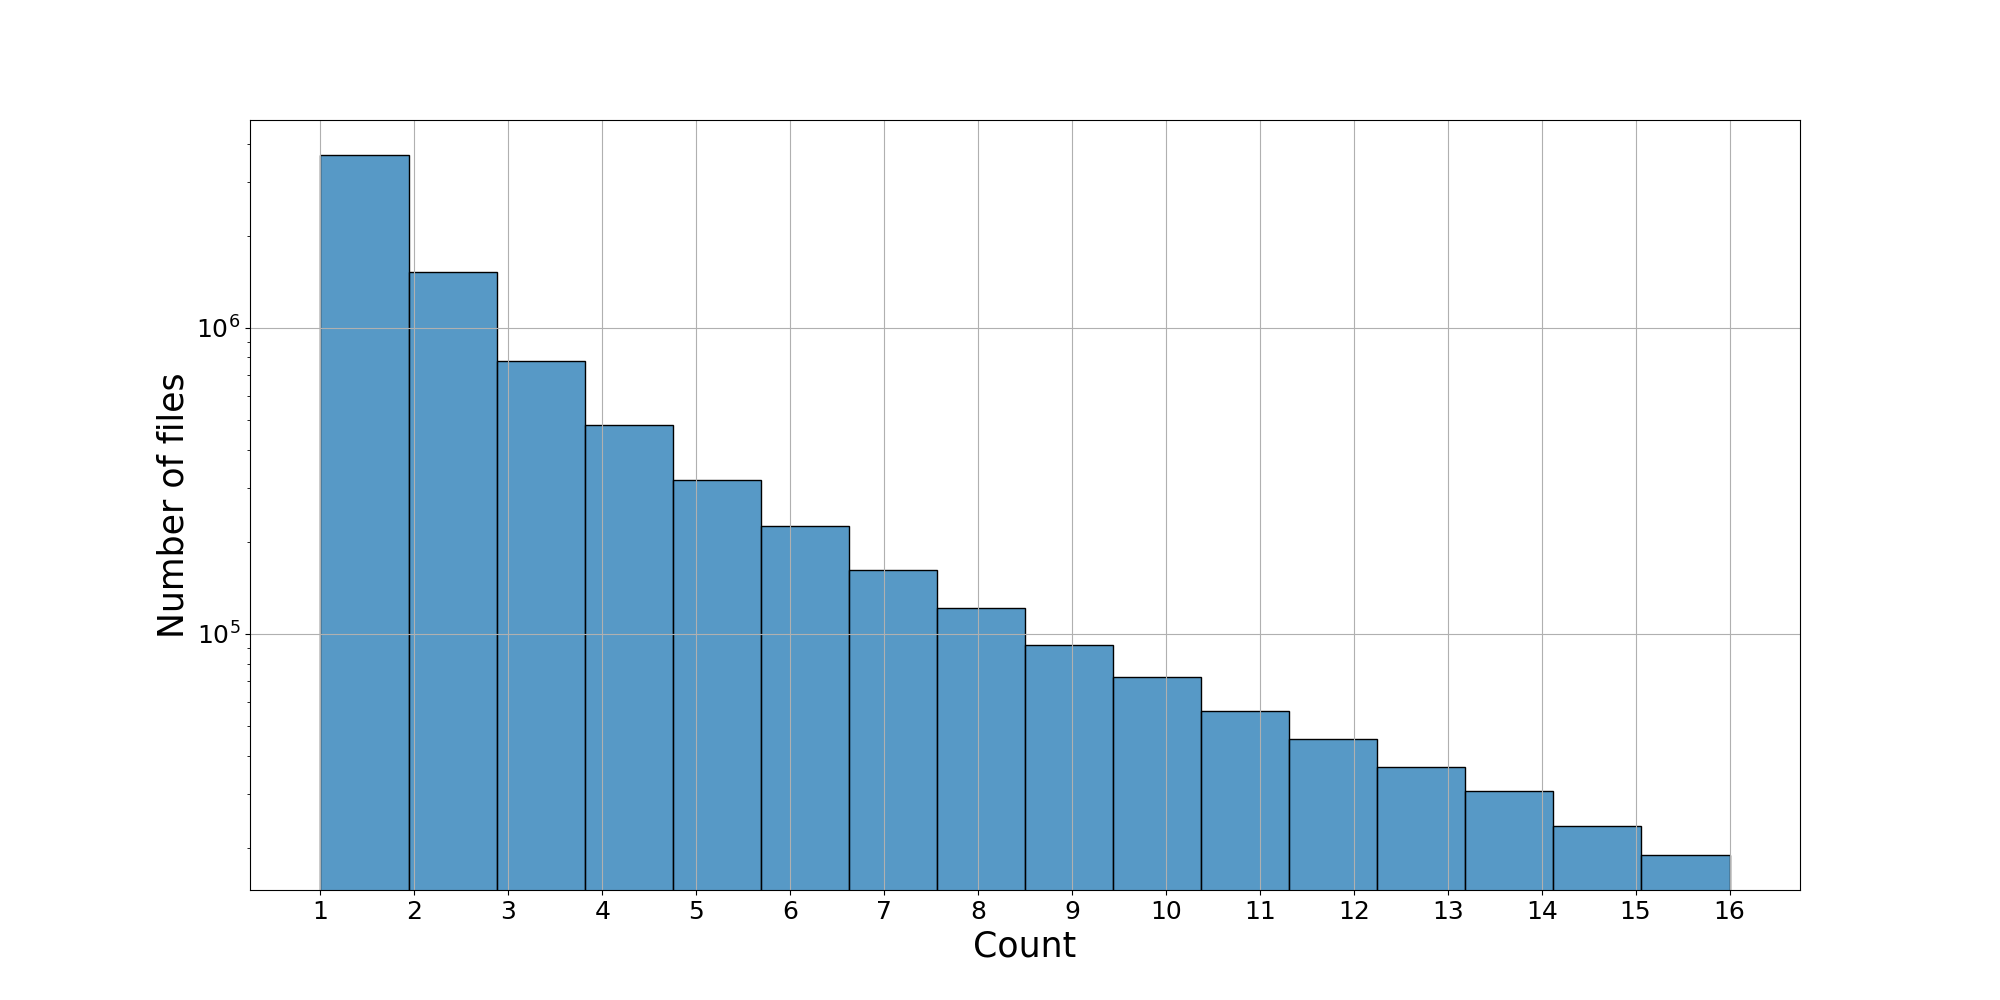
\includegraphics[scale=0.30]{figs/Commit num files distribution_comchron.png}
    \caption{Distribution of the number of files in commits in CommitChronicle.}~\label{fig:num_files_dist_CommitChronicle}
\end{figure}

\begin{table}[h]
    \centering
    \caption{Distribution of commit messages}\label{tab:commit_messages_CommitChronicle}
    \begin{tabular}{|l|r|} % chktex 44
    \hline % chktex 44
    \textbf{Commit Message} & \textbf{Count} \\ 
    \hline % chktex 44
    Add       & 541205 \\ \hline % chktex 44
    Fix       & 427753 \\ \hline % chktex 44
    Update    & 251594 \\ \hline % chktex 44
    add       & 198032 \\ \hline % chktex 44
    fix       & 177001 \\ \hline % chktex 44
    Added     & 158065 \\ \hline % chktex 44
    Remove    & 157336 \\ \hline % chktex 44
    fix:      & 118704 \\ \hline % chktex 44
    Use       & 93908  \\ \hline % chktex 44
    Fixed     & 89186  \\ \hline % chktex 44
    \end{tabular}
\end{table}

\begin{figure}[H]
    % \hspace*{-2.5cm}
    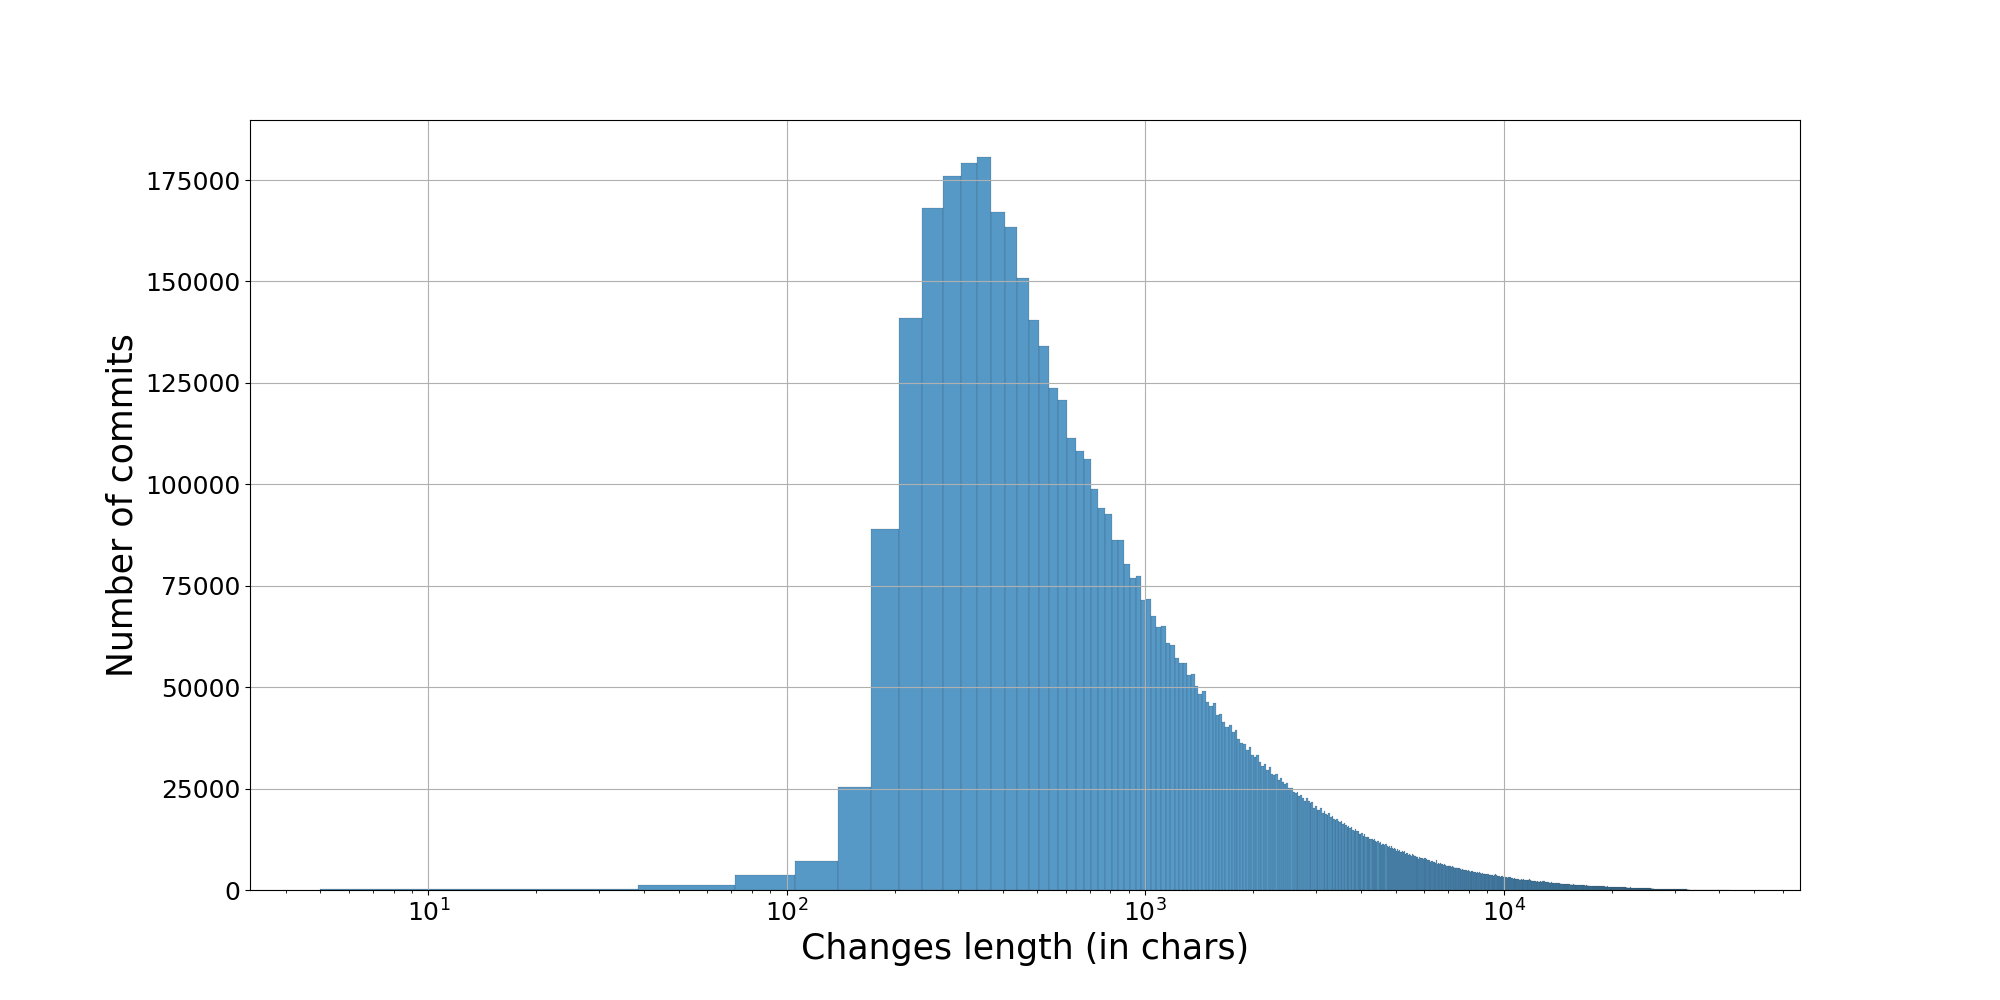
\includegraphics[scale=0.30]{figs/changes_len_dist_comchron.png}
    \caption{Distribution of length of commits in CommitChronicle.}~\label{fig:changes_len_dist_CommitChronicle}
\end{figure}

\begin{figure}[H]
    % \hspace*{-2.5cm}
    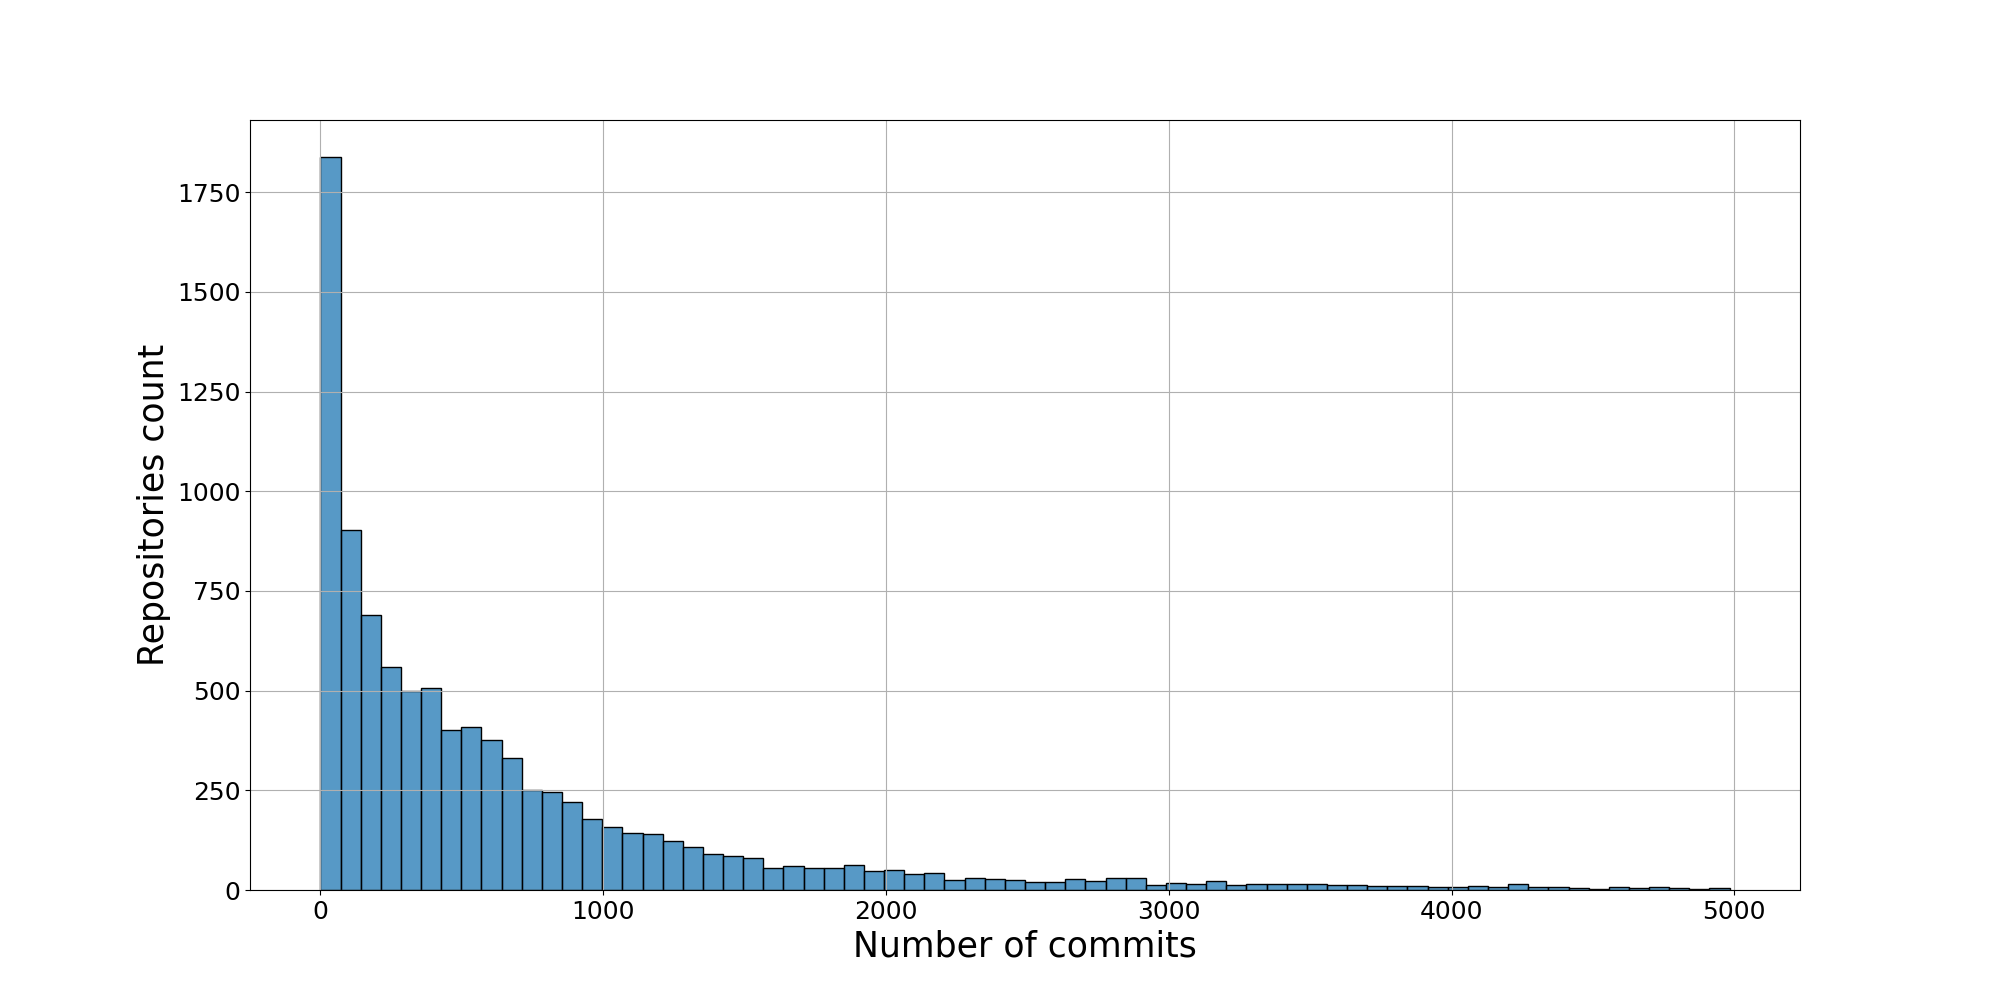
\includegraphics[scale=0.30]{figs/Commits distribution_comchron.png}
    \caption{Number of commits in the repositories in CommitChronicle.}~\label{fig:commits_distribution_CommitChronicle}
\end{figure}

\section{Conclusion about the data}
In this section, I would like to make the choice of the data used for the model training, evaluation and testing. From the data analysis, I got that CommitChronicle has a better representation of the data. It also has much more samples. So, it will be logical to use CommitChronicle as a train set. As a validation set, I will use a validation split of the CommitChronicle to be sure that I have no repetitive samples with the train data. For the test of my models, I will utilize both my custom dataset and the test split of CommitChronicle. The results of the models in the custom dataset may be represented as the results of out-of-domain data, as the process of getting the data differs, and some samples filtered out from CommitChronicle may be included.  So, this testing will examine the fair performance of the model in the `real world data`.

\section{CodeT5+ training}\label{sec:codeT5_train}
My first attempt at approaching the task of commit message generation is straightforward. I will consider this task as a simple NMT (Neural Machine Translation) problem. In this setting, the model aims to translate the input code into a natural language description of the code changes. The current SOTA solutions in the NMT task utilize the transformer architecture approach presented in~\cite{vaswani2017attention}. According to the specific domain of the input data for my task, the best choice is the model pre-trained on the massive amount of code. The model used as a backbone in the current SOTA solution of the CMG task presented at~{}\cite{eliseeva2023commit} is codeT5. The model was pre-trained on a variety of coding tasks and demonstrated proficient performance in code comprehension. However, since that time, the authors of CodeT5 have introduced an updated version of the model, called CodeT5+~\cite{wang2023codet5+}. This new model outperforms CodeT5 in performance across the majority of code-related benchmarks. So, I decided to train CodeT5+ on CMG task as the first experiment in my work. In this setting, I will use code difference from the commit as plain text. \\
As mentioned in Section~\ref{sec:CMG_approaches}, the most common method for generating commit messages involves representing both the input and output as a sequence of numerical tokens. In Paragraph~\ref{sec:structure_of_the_data}, I described the specific format of the input and output data for my task. Therefore, before training the model, it is necessary to add special tokens to the tokenizer vocabulary. The model will learn the embedded representation of these special tokens during training. This step will aid the model in better understanding the structure of code changes.
\begin{align}
    \label{eq:CrossEntropy}
    L(y, \hat{y}) = -\sum_{i=1}^{C} \log \left( \frac{e^{\hat{y_i}}}{\sum_{j=1}^{C} e^{\hat{y_{j}}}} \right) \times y_{i}
\end{align}

The loss function that should be optimized by the neural network is cross entropy loss represented at~\ref{eq:CrossEntropy}. $y$ here represents the true probability distribution of the next token choice from the tokenizer vocabulary in the target sequence. This is a vector with 1 in one position, and 0 in all the others, as we exactly know what token should come next. And $\hat{y}$ is the predicted vector of probability distribution to choose the next token.  This function tends to make the predicted vector as similar to the true vector as possible, \textit{i.e.} predict the next token correctly. Predicting the next token in an autoregressive manner model will generate a commit message for the given code edits. 

\section[Larger model experiments]{Experiments with larger CodeT5+}\label{sec:larger_model_experiments}
To assess the impact of scaling the model in terms of parameters on the quality of generated commits, I trained the CodeT5+ model with 770 million parameters. The differences between the base version and this model are presented in Table~\ref{tab:220_vs_770_compare}. From this table, it is clear that the distinctions between these models are primarily in the hidden representations and the number of blocks in both the encoder and decoder parts. A larger model version does not process longer sequences but has better internal representation, potentially enabling the generation of better commit messages. The training objective I utilized and the data format are identical to those used for training the base CodeT5+. This experiment demonstrated how scaling the depth of the neural network and improving representation can affect model performance. Additionally, this phase allowed me to determine whether 220 million parameters are sufficient for constructing commit messages that are relatively simple sequences. The final aspect requiring analysis in this section is how this scaling influences the model's inference time since efficiency in terms of time is as crucial as message quality when considering real-world applications.

\begin{table}[h]
    \centering
    \caption{Сomparison of CodeT5+ with 220M and 770M parameters}\label{tab:220_vs_770_compare}
    \renewcommand{\arraystretch}{1.5} % Adjusts the row height
    \begin{tabular}{|l|c|c|} % chktex 44
    \hline % chktex 44
    \textbf{Feature} & \textbf{220M model} & \textbf{770M model} \\ 
    \hline % chktex 44
    Context window tokens       & 512 & 512 \\ \hline % chktex 44
    Hidden state dimension       & 768 & 1024 \\ \hline % chktex 44
    Encoder transformer blocks    & 12 & 24 \\ \hline % chktex 44
    Decoder transformer blocks       & 12 & 24 \\ \hline % chktex 44
    Embedding dimension       & 32100 & 32100 \\ \hline % chktex 44
    \end{tabular}
\end{table}

\section{CodeT5+ with retrieval components training}\label{sec:codeT5_with_retrieval_train}
One of the problem with the traditional language modeling approach to the task of commit messages generation is the shared style of messages within the same repository. For example, repository of linux kernel source code have a strictly specified format of commit messages. Using only code modificaions it is impossible to adapt generated commit message to have the same spcified format. 

\subsection{Retrieval approaches}\label{subsec:retrieval_existing_methods}
To mitigate issue with a message style, works like~\cite{shi2022race},~\cite{liu2020atom}, and~\cite{wang2021context} adopt additinal retrieval module to the standard endcoder-decoder architecture. These methods are mostly uses the database of commits and corresponding commit message. And then new commit is given as an input to the model, this method firstly use encoder to get a embedded vector representation of code modifications. This representation is further used to find the most similar code changes from the dataset, and get both modifications and commit message. This additional information is then passed to the model to get the result. Analysis of these method shows, that retrieval mechanism leverages the results of commit generation. 

One more way to use the historical data in generation of commit messages is to retrieve previous commits from the same repository, or previous commits of the same person. This method way used in the~\cite{eliseeva2023commit}, and showed improvement of model performance. If previous methods are mostly used to improve the understanding of code changes, then this historical data retrieval method is used only for message style adaptation.   

\subsection{My experiment with retrieval}\label{subsec:retrieval_arch_method}
For my experiment, I decided on the method combining retrieving the most similar code modifications and getting historical data from the previous commits. My experiment is close to the one provided in~\cite{eliseeva2023commit} with a combination of the RACE method from~\cite{shi2022race} and the history of messages added to the model input. The main difference between my approach and the RACE  is that the RACE leverage the commit generation by passing the combination of the input code changes with the most similar one from the database. At the same time, my approach is utilizing only the message from the most similar commit to adapt to the style of the commit message of the same code theme.  Additionally, I pass to the model input history samples of the messages from the same repository. In the end, my input to the model have the following format:  
\begin{verbatim}
    <commit_msg> most simmilar message </commit_msg> 
    <commit_msg> previous message </commit_msg>
    code modifications 
\end{verbatim}
Generally, I construct my pipeline in the following manner. Firstly, I need to get the database from which I will retrieve the most similar commit. As a database, I used my training data. The similarity metric for my retrieval process is the cosine distance between the target embedding and embeddings from the dataset. For getting the embeddings of my data, I need the model pre-trained to understand code modifications and commit messages. For this purpose, I used a separated encoder part of the CodeT5+ fine-tuned for commit generation from my initial experiment. After the training on the large dataset of code changes, it should be able to construct meaningful embeddings. With the usage of the hidden states from the encoder, I extended my training data with the corresponding embeddings of code changes that I will further refer to as the database. One additional extension to the dataset is the previous commit message from the same repository. To obtain the message history, the training data was grouped by repositories and sorted in historical order based on commit timestamps. The model's forward pass involves running input code modifications through the encoder of the codeT5+ model to obtain embedded representations of input code changes. After calculating the embedding, I searched for the most similar one in the database and retrieved its commit message.

An important detail in the search process is to track the timestamp of a similar commit and the similarity of embeddings.  During the training process, the model takes a sample from the search database. Therefore, the most similar commit will always be its exact copy with the real commit message, as we have its copy in the search space. This behaviour will break the logic behind the method and lead our model to overfit, thus we should handle this situation and consider a threshold on the similarity for it not to be too big. One more restriction on the similar commit search is the timestamp of the retrieved sample. In the training phase model must not have access to the commits from the future.  This may cause a situation of retrieving the future commit from the same repository, changing the same piece of code, and leading the model to overfitting. Therefore I restricted my search space to the most similar sample with the similarity threshold and commits made only before the input one.  

With the help of the retrieved commit message and the history of the previous commits from the repository, I'm constructing the input in the format described above. These modifications will enhance the generated commit message adaptation to the repository's overall style and code change themes, thereby improving the text-matching metrics.





\section{Possible way to resolve limited context window problem}\label{sec:file_attention_arch}
TODO

\section{Metrics to evaluate CMG results}
In the literature review section, I have described the most popular metrics to measure the performance of the models in terms of generated commit message quality~\ref{sec:eval_metrics}. For my experiments, I used bath metrics described in the literature review. BLEU for the syntax similarity and BERTScore to access the semantic similarity with the original commit message. In this chapter, I aim to give an extensive definition of these metrics and the intuition behind them.

\subsection{BLEU score description}\label{subsec:bleu}
Bilingual evaluation understudity (\textbf{Bleu}) is the metric invented in 2002 and presented at~\cite{papineni2002bleu}. The original goal of this metric was to evaluate the quality of machine translation. The task of generating commit messages from code modifications is considered a translation from code to natural language. The original commit message in this setup is the reference translation. A comparison of the generated commit message with the original one matches the idea of the BLEU\@. Therefore, the results of this metric properly reflect the quality of the generated commit message. 

Considering details of this metric, its mathematical formulation is presented in formulas~\ref{formula:ngram_precision}-\ref{formula:bleu}. The final formula for the BLEU score shown in~\ref{formula:bleu}, is calculated as a product of brevity penalty (\textbf{BP}) and the weighted sum of n-gram precision. Bravity penalty is calculated according to the formula~\ref{formula:brave_penalty} and penalizes metric for too long generated text. In this formula $r$ stands for the length of generated text and $c$ is the length of the reference. The precision of the n-grams formula presented at~\ref{formula:ngram_precision} calculates the ratio matched n-grams to the total number of n-grams in the reference text for each sentence. Default parameters for BLEU score is $N=4$ and uniformly distributed $w_n = \frac{1}{4}$

\begin{align}\label{formula:ngram_precision}
    p_n = \frac{\sum_{\mathcal{C} \in \text{\{Candidates\}}} \sum_{\text{n-gram} \in \mathcal{C}} Count_{clip}(\text{n-gram})}
    {\sum_{\mathcal{C}' \in \text{\{Candidates\}}} \sum_{\text{n-gram}' \in \mathcal{C}'} Count(\text{n-gram}')}
\end{align}

\begin{align}\label{formula:brave_penalty}
    BP = \begin{cases}
        1 & \text{if } c > r \\ 
        e^{1 - r/c} & \text{if } c \leq r
    \end{cases}
\end{align}

\begin{align}\label{formula:bleu}
    BLEU_N = BP \times \exp{\left( \sum_{n=1}^{N} w_n \log p_n\right)}
\end{align}

From the explanation above, it is clear that the formula for BLEU strongly depends on configured parameters, n-grams $N$, and importance weights $w_n$. That makes this metric variative, and therefore, it is hard to compare the results among different works. To overcome this problem, the authors of~\cite{post2018call} presented the package SacreBLEU\@. This Python script helps calculate the BLEU score in a unified way to have reproducible results.

Analyzing the BLEU score specifically for the commit messages generation task, results from~\cite{tao2021evaluation} show that in this specific task related to code, it is more representative to use a normalized version of BLEU called B-Norm. The difference from the original method is to first convert both prediction and reference to lowercase, as it is not as important for this task, as for translation. The second difference is to add one to both the numerator and denominator of~\ref{formula:ngram_precision} to add smoothness to it.

In my experiments, I decided to use both SacreBLEU and B-Norm. This will make the results of the evaluation more extensive and fair. Counting SacreBLEU will help me compare my results with other approaches to solving CMG tasks. B-Norm is mostly used in my work to compare results with the work of JetBrains research~\cite{eliseeva2023commit}, as I used their method as a baseline for my work. To make a fair comparison in terms of B-Norm, I used the script to calculate the metrics from the source code of~\cite{eliseeva2023commit}, as it is open and free to use.

\subsection{BERTScore description}\label{subec:bertscore}
BERTScore is the metric for automatic evaluation of text generation presented at~\cite{zhang2019bertscore}. This metric is based on the BERT~\cite{devlin2018bert} {-} encoder-only transformer-based model. It was shown that the BERT model achieves outstanding results in encoding text and getting meaningful hidden representation. Utilizing this fact, BERTScore gets embeddings for each token of both generated text and reference. Due to the transformer-based architecture, the representation of the tokens may differ depending on the surrounding context. This feature makes this metric more representative than the BLEU score, which considers only matching n-grams, \textit{i.e.}, based only on the syntax similarity between generated text and reference. At the same time, BERTScore depends on the context and meaning of the word, therefore can catch the situation, then we have generated text with the same meaning, but written in other words.

Suppose we have reference text $x = \langle x_1, x_2 \dots x_k \rangle$ and generated candidate text $\hat{x} = \langle \hat{x_1}, \hat{x_2} \dots \hat{x_k} \rangle$ represented in tokens. The first step to calculate the BERTScore is to get embeddings of size $h$ of each token for both texts, resulting in two embeddings matrices $H_x \in \mathbb{R}^{k \times h}$ for the reference text and $H_{\hat{x}} \in \mathbb{R}^{l \times h}$ for the generated text. Further is to calculate cosine similarity for each hidden vector from matrices. Cosine similarity between reference token $x_i$ and candidate token $\hat{x_j}$ calculated as shown in~\ref{formula:cosine_sim}. The result of cosine similarity lies in the interval $[-1, 1]$ and represents the cosine of the angle between these two vectors. The closer these vectors are, the closer the cosine similarity to one.

\begin{align}\label{formula:cosine_sim}
    s = \frac{x_i^T x_j}{\|x_i\| \|\hat{x_j}\|}
\end{align}\\
Constructing a similarity matrix from pairwise cosine similarity of tokens I get matrix $S \in \mathbb{R}^{k \times l}$. One more detail about this metric is the importance of weighting for each token in the reference text. For this, the authors of this method used inverse document frequency (idf) scoring. Given M reference sentences $\{ x^{(i)} \}_{i=1}^M$ idf score for the token $w$ calcualted according to the~\ref{formula:idf}. 

\begin{align}\label{formula:idf}
    \text{idf}(w) = -\log \frac{1}{M} \sum_{i=1}^{M} \mathbb{I}\left[ w \in x^{(i)} \right]
\end{align}\\
Complete BERTScore matches each token in $x$ to a token in $\hat{x}$ to compute recall~\ref{formula:bert_recall}, and each token of $\hat{x}$ to a token in $x$ to calculate precision~\ref{formula:bert_precision}. The authors used a greedy strategy for token matching. Each token is matched to the most similar token in the other text. 

\begin{align}\label{formula:bert_recall}
    R_{BERT} = \frac{\sum_{x_i \in x } \text{idf}(x_i) \max_{x_j \in \hat{x}} x_i^T x_j}{\sum_{x_i \in x} \text{idf}(x_i)}
\end{align}

\begin{align}\label{formula:bert_precision}
    P_{BERT} = \frac{\sum_{x_j \in \hat{x} } \text{idf}(x_j) \max_{x_i \in x} x_i^T x_j}{\sum_{x_j \in \hat{x}} \text{idf}(x_j)}
\end{align}\\
For my experiment, I used the F1 score~\ref{formula:bert_f1}. It is calculated as a doubled geometric mean of precision and recall, thus including information from both these metrics. 
\begin{align}\label{formula:bert_f1}
    F_{BERT} = 2\frac{P_{BERT} \times R_{BERT}}{P_{BERT} + R_{BERT}}
\end{align}\\
The last important point about the BERTScore metric is the sensitivity to the base BERT model. As was written before, the most important step in calculating this metric is to get representative embedding for each of the tokens with BERT\@. And the choice for this is crucial to get an informative metric. For my experiments, I got deberta-xlarge-mnli from~\cite{he2021deberta}. The reason I choose this exact model is that authors of the evaluate\footnote[1]{\href{https://huggingface.co/docs/evaluate/index}{Evaluate - library with the implementation of the most modern ML metrics.}} library, have analyzed\footnote[1]{\href{https://huggingface.co/spaces/evaluate-metric/bertscore}{Documentation for BERTScore from evaluate}} the performance of most popular encoder models and states, that this version of DeBERTa shows the best performance for calculating the BERTScore.